%
% 6.006 problem set 0 solutions template
%
\documentclass[11pt,twoside]{article}

\newcommand{\name}{}

\usepackage{amssymb}
\usepackage{amsmath}
\usepackage{graphicx}
\usepackage{latexsym}
\usepackage{times,url}
\usepackage{cprotect}
\usepackage{listings}
\usepackage{graphicx}
\usepackage[table]{xcolor}
\usepackage[letterpaper]{geometry}
\usepackage{tikz-qtree}
\usepackage{enumerate}

\newcommand{\profs}{Instructors: Dr. Nadi}
\newcommand{\subj}{6.006}
\newcommand{\ttt}[1]{{\tt\small #1}}

\definecolor{dkgreen}{rgb}{0,0.6,0}
\definecolor{dkblue}{rgb}{.2,.2,1}
\definecolor{gray}{rgb}{0.5,0.5,0.5}
\definecolor{mauve}{rgb}{0.58,0,0.82}

\lstset{
  language=Python,
  aboveskip=1pc,
  belowskip=1pc,
  basicstyle={\footnotesize\ttfamily},
  numbers=left,
  showstringspaces=false,
  numberstyle={\tiny\color{gray}\ttfamily},
  keywordstyle={\color{dkblue}\ttfamily},
  commentstyle={\color{dkgreen}\ttfamily},
  stringstyle={\color{mauve}\ttfamily},
}

% \lstset{
%   language=Python,
%   aboveskip=1pc,
%   belowskip=1pc,
%   basicstyle={\bf\color{white}\ttfamily},
%   numbers=left,
%   showstringspaces=false,
%   numberstyle={\bf\small\color{lightgray}\ttfamily},
%   keywordstyle={\bf\color{cyan}\ttfamily},
%   commentstyle={\bf\color{green}\ttfamily},
%   stringstyle={\bf\color{mauve}\ttfamily},
% }

\tikzset{
  % every node/.style={minimum width=2em,draw,circle},
  % level 1/.style={sibling distance=2cm},
  level distance=1cm,
  edge from parent/.style=
  {draw,edge from parent path={(\tikzparentnode) -- (\tikzchildnode)}},
}
\usetikzlibrary{shapes}

\newif\ifHideSolutions
\newcommand{\solutionBL}[1]{\textbf{Solution: }#1\color{black}}

\newif\ifHideSolutions
\newcommand{\solution}[1]{\color{dkgreen}\textbf{Solution: }#1\color{black}}
\newcommand{\commonmistakes}[1]{{\color{dkblue}\textbf{Common Mistakes: }#1}}
\newcommand{\rubric}[1]{\color{dkgreen}{\bf Rubric:} #1\color{black}}

% \HideSolutionsfalse
% \ifHideSolutions
%   \renewcommand{\solution}[1]{}
%   \renewcommand{\rubric}[1]{}
% \fi

\newlength{\toppush}
\setlength{\toppush}{2\headheight}
\addtolength{\toppush}{\headsep}

\newcommand{\htitle}[2]{\noindent\vspace*{-\toppush}\newline\parbox{0.5 \textwidth}
{\textit{Experiential Learning}\hfill   \name\newline
University of Tehran \hfill\newline
\profs 
\\[-3.5ex]\newline
}
\begin{minipage}{0.5\textwidth}
  \raggedleft % Equivalent to \flushright but often used in minipage for clarity
    \vspace{-0.37cm}
\includegraphics[width=1.75cm]{fig/Tehran-Uni-logo.png}\hspace*{0.22cm}
\end{minipage}
\mbox{}\hrulefill\mbox{}
\mbox{}\newline
\begin{center}{\Large\bf #1}\end{center}}

\newcommand{\handout}[2]{\thispagestyle{empty}
 \markboth{#1}{#1}
 \pagestyle{myheadings}\htitle{#1}{#2}}

\newcommand{\lecture}[3]{\thispagestyle{empty}
 \markboth{Lecture #1: #2}{Lecture #1: #2}
 \pagestyle{myheadings}\htitle{Lecture #1: #2}{#3}}

\newcommand{\htitlewithouttitle}[2]{\noindent\vspace*{-\toppush}\newline\parbox{6.5in}
{\textit{Introduction to Algorithms}\hfill#2\newline
Massachusetts Institute of Technology \hfill 6.006\newline
\profs\hfill Handout #1\vspace*{-.5ex}\newline
\mbox{}\hrulefill\mbox{}}\vspace*{1ex}\mbox{}\newline}

\newcommand{\handoutwithouttitle}[2]{\thispagestyle{empty}
 \markboth{Handout \protect\ref{#1}}{Handout \protect\ref{#1}}
 \pagestyle{myheadings}\htitlewithouttitle{\protect\ref{#1}}{#2}}

\newcommand{\exam}[2]{% parameters: exam name, date
 \thispagestyle{empty}
 \markboth{\hspace{1cm}\subj\ #1\hspace{1in}Name\hrulefill\ \ }%
          {\subj\ #1\hspace{1in}Name\hrulefill\ \ }
 \pagestyle{myheadings}\examtitle{#1}{#2}
 \renewcommand{\theproblem}{Problem \arabic{problemnum}}
}
\newcommand{\examsolutions}[3]{% parameters: handout, exam name, date
 \thispagestyle{empty}
 \markboth{Handout \protect\ref{#1}: #2}{Handout \protect\ref{#1}: #2}
% \pagestyle{myheadings}\htitle{\protect\ref{#1}}{#2}{#3}
 \pagestyle{myheadings}\examsolutionstitle{\protect\ref{#1}} {#2}{#3}
 \renewcommand{\theproblem}{Problem \arabic{problemnum}}
}
\newcommand{\examsolutionstitle}[3]{\noindent\vspace*{-\toppush}\newline\parbox{6.5in}
{\textit{Introduction to Algorithms}\hfill#3\newline
Massachusetts Institute of Technology \hfill 6.006\newline
%Singapore-MIT Alliance \hfill SMA5503\newline
\profs\hfill Handout #1\vspace*{-.5ex}\newline
\mbox{}\hrulefill\mbox{}}\vspace*{1ex}\mbox{}\newline
\begin{center}{\Large\bf #2}\end{center}}

\newcommand{\takehomeexam}[2]{% parameters: exam name, date
 \thispagestyle{empty}
 \markboth{\subj\ #1\hfill}{\subj\ #1\hfill}
 \pagestyle{myheadings}\examtitle{#1}{#2}
 \renewcommand{\theproblem}{Problem \arabic{problemnum}}
}

\makeatletter
\newcommand{\exambooklet}[2]{% parameters: exam name, date
 \thispagestyle{empty}
 \markboth{\subj\ #1}{\subj\ #1}
 \pagestyle{myheadings}\examtitle{#1}{#2}
 \renewcommand{\theproblem}{Problem \arabic{problemnum}}
 \renewcommand{\problem}{\newpage
 \item \let\@currentlabel=\theproblem
 \markboth{\subj\ #1, \theproblem}{\subj\ #1, \theproblem}}
}
\makeatother


\newcommand{\examtitle}[2]{\noindent\vspace*{-\toppush}\newline\parbox{6.5in}
{\textit{Introduction to Algorithms}\hfill#2\newline
Massachusetts Institute of Technology \hfill 6.006 Spring 2020\newline
%Singapore-MIT Alliance \hfill SMA5503\newline
\profs\hfill #1\vspace*{-.5ex}\newline
\mbox{}\hrulefill\mbox{}}\vspace*{1ex}\mbox{}\newline
\begin{center}{\Large\bf #1}\end{center}}

\newcommand{\grader}[1]{\hspace{1cm}\textsf{\textbf{#1}}\hspace{1cm}}

\newcommand{\points}[1]{[#1 points]\ }
\newcommand{\parts}[1]
{
  \ifnum#1=1
  (1 part)
  \else
  (#1 parts)
  \fi
  \ 
}

\newcommand{\bparts}{\begin{problemparts}}
\newcommand{\eparts}{\end{problemparts}}
\newcommand{\ppart}{\problempart}

%\newcommand{\lg} {lg\ }

\setlength{\oddsidemargin}{0pt}
\setlength{\evensidemargin}{0pt}
\setlength{\textwidth}{6.5in}
\setlength{\topmargin}{0in}
\setlength{\textheight}{8.5in}


\newcommand{\Spawn}{{\bf spawn} }
\newcommand{\Sync}{{\bf sync}}

\newcommand{\cif}[1]{\mbox{if $#1$}}
\newcommand{\cwhen}[1]{\mbox{when $#1$}}

\newcounter{problemnum}
\newcommand{\theproblem}{Problem \arabic{problemnum}}
\newenvironment{problems}{
        \begin{list}{{\bf \theproblem. \hspace*{0.5em}}}
        {\setlength{\leftmargin}{0em}
         \setlength{\rightmargin}{0em}
         \setlength{\labelwidth}{0em}
         \setlength{\labelsep}{0em}
         \usecounter{problemnum}}}{\end{list}}
\makeatletter
\newcommand{\problem}[1][{}]{\item \let\@currentlabel=\theproblem \textbf{#1}}
\makeatother

\newcounter{problempartnum}[problemnum]
\newenvironment{problemparts}{
        \begin{list}{{\bf (\alph{problempartnum})}}
        {\setlength{\leftmargin}{2.5em}
         \setlength{\rightmargin}{2.5em}
         \setlength{\labelsep}{0.5em}}}{\end{list}}
\newcommand{\problempart}{\addtocounter{problempartnum}{1}\item}

\newenvironment{truefalseproblemparts}{
        \begin{list}{{\bf (\alph{problempartnum})\ \ \ T\ \ F\hfil}}
        {\setlength{\leftmargin}{4.5em}
         \setlength{\rightmargin}{2.5em}
         \setlength{\labelsep}{0.5em}
         \setlength{\labelwidth}{4.5em}}}{\end{list}}

\newcounter{exercisenum}
\newcommand{\theexercise}{Exercise \theproblemsetnum-\arabic{exercisenum}}
\newenvironment{exercises}{
        \begin{list}{{\bf \theexercise. \hspace*{0.5em}}}
        {\setlength{\leftmargin}{0em}
         \setlength{\rightmargin}{0em}
         \setlength{\labelwidth}{0em}
         \setlength{\labelsep}{0em}
        \usecounter{exercisenum}}}{\end{list}}
\makeatletter
\newcommand{\exercise}{\item \let\@currentlabel=\theexercise}
\makeatother

\newcounter{exercisepartnum}[exercisenum]
%\newcommand{\problem}[1]{\medskip\mbox{}\newline\noindent{\bf Problem #1.}\hspace*{1em}}
%\newcommand{\exercise}[1]{\medskip\mbox{}\newline\noindent{\bf Exercise #1.}\hspace*{1em}}

\newenvironment{exerciseparts}{
        \begin{list}{{\bf (\alph{exercisepartnum})}}
        {\setlength{\leftmargin}{2.5em}
         \setlength{\rightmargin}{2.5em}
         \setlength{\labelsep}{0.5em}}}{\end{list}}
\newcommand{\exercisepart}{\addtocounter{exercisepartnum}{1}\item}


% Macros to make captions print with small type and 'Figure xx' in bold.
\makeatletter
\def\fnum@figure{{\bf Figure \thefigure}}
\def\fnum@table{{\bf Table \thetable}}
\let\@mycaption\caption
%\long\def\@mycaption#1[#2]#3{\addcontentsline{\csname
%  ext@#1\endcsname}{#1}{\protect\numberline{\csname 
%  the#1\endcsname}{\ignorespaces #2}}\par
%  \begingroup
%    \@parboxrestore
%    \small
%    \@makecaption{\csname fnum@#1\endcsname}{\ignorespaces #3}\par
%  \endgroup}
%\def\mycaption{\refstepcounter\@captype \@dblarg{\@mycaption\@captype}}
%\makeatother
\let\mycaption\caption
%\newcommand{\figcaption}[1]{\mycaption[]{#1}}

\newcounter{totalcaptions}
\newcounter{totalart}

\newcommand{\figcaption}[1]{\addtocounter{totalcaptions}{1}\caption[]{#1}}

% \psfigures determines what to do for figures:
%       0 means just leave vertical space
%       1 means put a vertical rule and the figure name
%       2 means insert the PostScript version of the figure
%       3 means put the figure name flush left or right
\newcommand{\psfigures}{0}
\newcommand{\spacefigures}{\renewcommand{\psfigures}{0}}
\newcommand{\rulefigures}{\renewcommand{\psfigures}{1}}
\newcommand{\macfigures}{\renewcommand{\psfigures}{2}}
\newcommand{\namefigures}{\renewcommand{\psfigures}{3}}

\newcommand{\figpart}[1]{{\bf (#1)}\nolinebreak[2]\relax}
\newcommand{\figparts}[2]{{\bf (#1)--(#2)}\nolinebreak[2]\relax}


\macfigures     % STATE

% When calling \figspace, make sure to leave a blank line afterward!!
% \widefigspace is for figures that are more than 28pc wide.
\newlength{\halffigspace} \newlength{\wholefigspace}
\newlength{\figruleheight} \newlength{\figgap}
\newcommand{\setfiglengths}{\ifnum\psfigures=1\setlength{\figruleheight}{\hruleheight}\setlength{\figgap}{1em}\else\setlength{\figruleheight}{0pt}\setlength{\figgap}{0em}\fi}
\newcommand{\figspace}[2]{\ifnum\psfigures=0\leavefigspace{#1}\else%
\setfiglengths%
\setlength{\wholefigspace}{#1}\setlength{\halffigspace}{.5\wholefigspace}%
\rule[-\halffigspace]{\figruleheight}{\wholefigspace}\hspace{\figgap}#2\fi}
\newlength{\widefigspacewidth}
% Make \widefigspace put the figure flush right on the text page.
\newcommand{\widefigspace}[2]{
\ifnum\psfigures=0\leavefigspace{#1}\else%
\setfiglengths%
\setlength{\widefigspacewidth}{28pc}%
\addtolength{\widefigspacewidth}{-\figruleheight}%
\setlength{\wholefigspace}{#1}\setlength{\halffigspace}{.5\wholefigspace}%
\makebox[\widefigspacewidth][r]{#2\hspace{\figgap}}\rule[-\halffigspace]{\figruleheight}{\wholefigspace}\fi}
\newcommand{\leavefigspace}[1]{\setlength{\wholefigspace}{#1}\setlength{\halffigspace}{.5\wholefigspace}\rule[-\halffigspace]{0em}{\wholefigspace}}

% Commands for including figures with macpsfig.
% To use these commands, documentstyle ``macpsfig'' must be specified.
\newlength{\macfigfill}
\makeatother
\newlength{\bbx}
\newlength{\bby}
\newcommand{\macfigure}[5]{\addtocounter{totalart}{1}
\ifnum\psfigures=2%
\setlength{\bbx}{#2}\addtolength{\bbx}{#4}%
\setlength{\bby}{#3}\addtolength{\bby}{#5}%
\begin{flushleft}
\ifdim#4>28pc\setlength{\macfigfill}{#4}\addtolength{\macfigfill}{-28pc}\hspace*{-\macfigfill}\fi%
\mbox{\psfig{figure=./#1.ps,%
bbllx=#2,bblly=#3,bburx=\bbx,bbury=\bby}}
\end{flushleft}%
\else\ifdim#4>28pc\widefigspace{#5}{#1}\else\figspace{#5}{#1}\fi\fi}
\makeatletter

\newlength{\savearraycolsep}
\newcommand{\narrowarray}[1]{\setlength{\savearraycolsep}{\arraycolsep}\setlength{\arraycolsep}{#1\arraycolsep}}
\newcommand{\normalarray}{\setlength{\arraycolsep}{\savearraycolsep}}

\newcommand{\hint}{{\bf Hint:\ }}

% Macros from /th/u/clr/mac.tex

\newcommand{\set}[1]{\left\{ #1 \right\}}
\newcommand{\abs}[1]{\left| #1\right|}
\newcommand{\card}[1]{\left| #1\right|}
\newcommand{\floor}[1]{\left\lfloor #1 \right\rfloor}
\newcommand{\ceil}[1]{\left\lceil #1 \right\rceil}
\newcommand{\ang}[1]{\ifmmode{\left\langle #1 \right\rangle}
   \else{$\left\langle${#1}$\right\rangle$}\fi}
        % the \if allows use outside mathmode,
        % but will swallow following space there!
\newcommand{\paren}[1]{\left( #1 \right)}
\newcommand{\bracket}[1]{\left[ #1 \right]}
\newcommand{\prob}[1]{\Pr\left\{ #1 \right\}}
\newcommand{\Var}{\mathop{\rm Var}\nolimits}
\newcommand{\expect}[1]{{\rm E}\left[ #1 \right]}
\newcommand{\expectsq}[1]{{\rm E}^2\left[ #1 \right]}
\newcommand{\variance}[1]{{\rm Var}\left[ #1 \right]}
\renewcommand{\choose}[2]{{{#1}\atopwithdelims(){#2}}}
\def\pmod#1{\allowbreak\mkern12mu({\rm mod}\,\,#1)}
\newcommand{\matx}[2]{\left(\begin{array}{*{#1}{c}}#2\end{array}\right)}
\newcommand{\Adj}{\mathop{\rm Adj}\nolimits}

\newtheorem{theorem}{Theorem}
\newtheorem{lemma}[theorem]{Lemma}
\newtheorem{corollary}[theorem]{Corollary}
\newtheorem{xample}{Example}
\newtheorem{definition}{Definition}
\newenvironment{example}{\begin{xample}\rm}{\end{xample}}
\newcommand{\proof}{\noindent{\em Proof.}\hspace{1em}}
\def\squarebox#1{\hbox to #1{\hfill\vbox to #1{\vfill}}}
\newcommand{\qedbox}{\vbox{\hrule\hbox{\vrule\squarebox{.667em}\vrule}\hrule}}
\newcommand{\qed}{\nopagebreak\mbox{}\hfill\qedbox\smallskip}
\newcommand{\eqnref}[1]{(\protect\ref{#1})}

%%\newcommand{\twodots}{\mathinner{\ldotp\ldotp}}
\newcommand{\transpose}{^{\mbox{\scriptsize \sf T}}}
\newcommand{\amortized}[1]{\widehat{#1}}

\newcommand{\punt}[1]{}

%%% command for putting definitions into boldface
% New style for defined terms, as of 2/23/88, redefined by THC.
\newcommand{\defn}[1]{{\boldmath\textit{\textbf{#1}}}}
\newcommand{\defi}[1]{{\textit{\textbf{#1\/}}}}

\newcommand{\red}{\leq_{\rm P}}
\newcommand{\lang}[1]{%
\ifmmode\mathord{\mathcode`-="702D\rm#1\mathcode`\-="2200}\else{\rm#1}\fi}

%\newcommand{\ckt}[1]{\ifmmode\mathord{\mathcode`-="702D\sc #1\mathcode`\-="2200}\else$\mathord{\mathcode`-="702D\sc #1\mathcode`\-="2200}$\fi}
\newcommand{\ckt}[1]{\ifmmode \sc #1\else$\sc #1$\fi}

%% Margin notes - use \notesfalse to turn off notes.
\setlength{\marginparwidth}{0.6in}
\reversemarginpar
\newif\ifnotes
\notestrue
\newcommand{\longnote}[1]{
  \ifnotes
    {\medskip\noindent Note: \marginpar[\hfill$\Longrightarrow$]
      {$\Longleftarrow$}{#1}\medskip}
  \fi}
\newcommand{\note}[1]{
  \ifnotes
    {\marginpar{\tiny \raggedright{#1}}}
  \fi}


\newcommand{\reals}{\mathbbm{R}}
\newcommand{\integers}{\mathbbm{Z}}
\newcommand{\naturals}{\mathbbm{N}}
\newcommand{\rationals}{\mathbbm{Q}}
\newcommand{\complex}{\mathbbm{C}}

\newcommand{\oldreals}{{\bf R}}
\newcommand{\oldintegers}{{\bf Z}}
\newcommand{\oldnaturals}{{\bf N}}
\newcommand{\oldrationals}{{\bf Q}}
\newcommand{\oldcomplex}{{\bf C}}

\newcommand{\w}{\omega}                 %% for fft chapter

\newenvironment{closeitemize}{\begin{list}
{$\bullet$}
{\setlength{\itemsep}{-0.2\baselineskip}
\setlength{\topsep}{0.2\baselineskip}
\setlength{\parskip}{0pt}}}
{\end{list}}

% These are necessary within a {problems} environment in order to restore
% the default separation between bullets and items.
\newenvironment{normalitemize}{\setlength{\labelsep}{0.5em}\begin{itemize}}
                              {\end{itemize}}
\newenvironment{normalenumerate}{\setlength{\labelsep}{0.5em}\begin{enumerate}}
                                {\end{enumerate}}

%\def\eqref#1{Equation~(\ref{eq:#1})}
%\newcommand{\eqref}[1]{Equation (\ref{eq:#1})}
\newcommand{\eqreftwo}[2]{Equations (\ref{eq:#1}) and~(\ref{eq:#2})}
\newcommand{\ineqref}[1]{Inequality~(\ref{ineq:#1})}
\newcommand{\ineqreftwo}[2]{Inequalities (\ref{ineq:#1}) and~(\ref{ineq:#2})}

\newcommand{\figref}[1]{Figure~\ref{fig:#1}}
\newcommand{\figreftwo}[2]{Figures \ref{fig:#1} and~\ref{fig:#2}}

\newcommand{\liref}[1]{line~\ref{li:#1}}
\newcommand{\Liref}[1]{Line~\ref{li:#1}}
\newcommand{\lirefs}[2]{lines \ref{li:#1}--\ref{li:#2}}
\newcommand{\Lirefs}[2]{Lines \ref{li:#1}--\ref{li:#2}}
\newcommand{\lireftwo}[2]{lines \ref{li:#1} and~\ref{li:#2}}
\newcommand{\lirefthree}[3]{lines \ref{li:#1}, \ref{li:#2}, and~\ref{li:#3}}

\newcommand{\lemlabel}[1]{\label{lem:#1}}
\newcommand{\lemref}[1]{Lemma~\ref{lem:#1}} 

\newcommand{\exref}[1]{Exercise~\ref{ex:#1}}

\newcommand{\handref}[1]{Handout~\ref{#1}}

\newcommand{\defref}[1]{Definition~\ref{def:#1}}

% (1997.8.16: Victor Luchangco)
% Modified \hlabel to only get date and to use handouts counter for number.
%   New \handout and \handoutwithouttitle commands in newmac.tex use this.
%   The date is referenced by <label>-date.
%   (Retained old definition as \hlabelold.)
%   Defined \hforcelabel to use an argument instead of the handouts counter.

\newcounter{handouts}
\setcounter{handouts}{0}

\newcommand{\hlabel}[2]{%
\stepcounter{handouts}
{\edef\next{\write\@auxout{\string\newlabel{#1}{{\arabic{handouts}}{0}}}}\next}
\write\@auxout{\string\newlabel{#1-date}{{#2}{0}}}
}

\newcommand{\hforcelabel}[3]{%          Does not step handouts counter.
\write\@auxout{\string\newlabel{#1}{{#2}{0}}}
\write\@auxout{\string\newlabel{#1-date}{{#3}{0}}}}


% less ugly underscore
% --juang, 2008 oct 05
\renewcommand{\_}{\vrule height 0 pt depth 0.4 pt width 0.5 em \,}

% multiline framed box (will always extend to the far right edge; for a short single line, use \fbox directly)
% --zabel, fall 2018
\newcommand\framepar[1]{\fbox{\begin{minipage}{\linewidth}#1\end{minipage}}}


\newcommand{\theproblemsetnum}{3}
\usepackage{xcolor}
\usepackage{caption}
\usepackage{geometry}
\usepackage{hyperref}
\usepackage{float}
\usepackage{booktabs} % For better horizontal rules
\usepackage{tabularx} % For flexibility in column widths
\usepackage{multirow}
\usepackage{array}
\usepackage{changepage} % for the adjustwidth environment
\usepackage{lipsum}
\usepackage{tikz}
\usepackage{adjustbox}
\usetikzlibrary{shapes, arrows.meta, positioning}
\usepackage{mathtools}
\usepackage{amsmath}
\usepackage{subcaption}

\newcommand{\labels}[2]{%
\\ \textcolor{cyan}{$#1+$}, \textcolor{magenta}{$#2-$}%
}

\setlength{\parskip}{0.5em} % Adjust to desired spacing

\title{UT ML Problem Set 2}

\begin{document}
\handout{Project Report}

\setlength{\parindent}{0pt}

\begin{center}

{\LARGE \textbf{An Overview of Language Models }} \\[20pt]

\textbf{ --- Fall 2024 --- } \\[15pt]

\medskip

{\large \textbf{Project Collaborators:}}
\medskip

\begin{table}[h]
\centering
\begin{tabularx}{0.8\textwidth}{>{\centering\arraybackslash}X >{\centering\arraybackslash}X}
\toprule
\textbf{Name} & \textbf{Student ID} \\
\midrule
Mobin Roohi & 610300060 \\
Amirhossein Ghorbaninezhad &  610xxxxxx\\
Vida Karbasi & 610xxxxxx \\
Ali Ghozati & 610xxxxxx \\
\bottomrule \\[20pt]
\end{tabularx}
\end{table}
\end{center}


\begin{abstract}
\textit{}

\textit{
}

\textit{
}

\textit{
}
\end{abstract}

\newpage

%%%%%%%%%%%%%%%%%%%%%%%%%%%%%%%%%%%%%%%%%%%%%%%%%%%%%
% See below for common and useful latex constructs. %
%%%%%%%%%%%%%%%%%%%%%%%%%%%%%%%%%%%%%%%%%%%%%%%%%%%%%

% Some useful commands:
% $f(x) = \Theta(x)$
% $T(x, y) \leq \log(x) + 2^y + \binom{2n}{n}$
% \ttt{code\_function}


% You can create unnumbered lists as follows:
% \begin{itemize}
%     \item First item in a list
%         \begin{itemize}
%             \item First item in a list
%                 \begin{itemize}
%                     \item First item in a list
%                     \item Second item in a list
%                 \end{itemize}
%             \item Second item in a list
%         \end{itemize}
%     \item Second item in a list
% \end{itemize}

% You can create numbered lists as follows:
% \begin{enumerate}
%     \item First item in a list
%     \item Second item in a list
%     \item Third item in a list
% \end{enumerate}

% You can write aligned equations as follows:
% \begin{align}
%     \begin{split}
%         (x+y)^3 &= (x+y)^2(x+y) \\
%                 &= (x^2+2xy+y^2)(x+y) \\
%                 &= (x^3+2x^2y+xy^2) + (x^2y+2xy^2+y^3) \\
%                 &= x^3+3x^2y+3xy^2+y^3
%     \end{split}
% \end{align}

% You can create grids/matrices as follows:
% \begin{align}
%     A =
%     \begin{bmatrix}
%         A_{11} & A_{21} \\
%         A_{21} & A_{22}
%     \end{bmatrix}
% \end{align}


%‌ PCA‌ %%%%%%%%%%%%%%%%%%%%%%%%%%%%%%%%%%%%%%%%%%%%%%%%%%

{
\setlength{\parskip}{0.35em} 
\tableofcontents
}
\newpage



\addcontentsline{toc}{section}{Bibliography}
\bibliographystyle{unsrt}
\bibliography{Biby.bib}

\section{Transformer Networks}

\subsection{Encoder-Decoder Architecture}
A common architecture in sequence-to-sequence models is the encoder-decoder architecture. In this architecture, generally, the model consists of an encoder component, which receives the input sequence and learns to encode it into complex representations. Then, a decoder component uses these representations from the encoder to generate the output sequence. Here, the decoder essentially acts as a conditional language model, taking in the encoded input from the encoder and the leftwards context of the target sequence and predicting the subsequent target sequence. 

Here is a diagram showing the encoder-decoder architecture:

\begin{figure}[h]
    \centering
    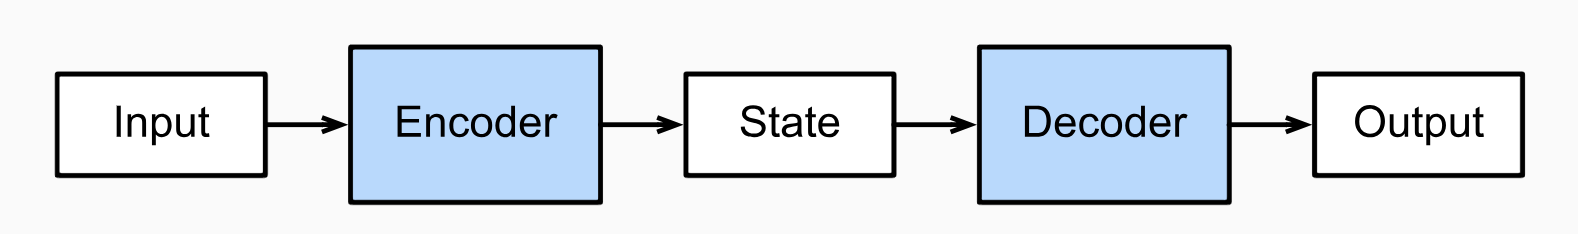
\includegraphics[width=0.65\linewidth]{fig/enc-dec.png}
    \caption{Encoder-Decoder Architecture}
\end{figure}

Encoder-decoder architectures can successfully be employed in sequence to sequence tasks with varying input and output sizes, such as machine translation, text summarization, and more. 

\textcolor{red}{[Dive Into Deep Learning]}

\subsection{Limitations of Recurrent Networks}
Recurrent neural networks \textcolor{red}{[Reference]}, long short-term memory \textcolor{red}{[Reference]}, gated recurrent \textcolor{red}{[Reference]}, and similar recurrent networks, have been firmly established well-performing approaches in sequence modeling and transduction problems such as language modeling, machine translation, and other NLP problems.

Recurrent models typically compute along the symbol positions of the input and output sequences. This means that they perform their computations sequentially. They learn a sequence of hidden states $h_t$ as a function of the previous hidden state $h_{t-1}$ and the input for position $t$. This sequential nature of processing limits parallelization within training examples, which becomes a problem with longer sequences as memory constraints limit batching across examples and training times increase. 

Moreover, these models can not quite capture the long-term dependencies and contexts of longer sequences. To mitigate these problems and improve model performance, a ground-breaking architecture called the Transformer Network was proposed in 2017 \textcolor{red}{[Transformer]}. The Transformer uses the following mechanisms in its architecture: \\[-20pt]
\begin{enumerate}
    \item Self-Attention \\[-20pt]
    \item Multi-Head Attention \\[-20pt]
    \item Positional Encoding \\[-20pt]
    \item Batch Norm \\[-20pt]
    \item Residual Connections \\[-20pt]
    \item Masked Multi-Head Attention \\[-20pt]
\end{enumerate}

We will first discuss some of these concepts briefly before providing the full Transformer architecture.

\subsection{Mechanisms in Transformer}
\subsubsection{Self-Attention}
To build up to the Transformer network, we need to first speak about its most fundamental component: \textbf{Self-Attention}.

Static Embeddings, as previously discussed, convert a token into a feature vector embedding that represents the token with a vector of numbers. Static embeddings, unfortunately, do not take the context of the token into account when creating the vector embedding. This is a limitation of the static embeddings learned using algorithms such as seq2vec.

To expand the idea of static embeddings to include contextualized information, self-attention is used to create contextualized embeddings that more adequately represent tokens in a sentence.

Self-attention inputs the input tokens ${X}$ and then uses three learnable weight matrices,

$$
\begin{align*}
&W^Q \in \mathbb{R}^{d_{\text {model }} \times d_k} \\ &W^K \in \mathbb{R}^{d_{\text {model }} \times d_k} \\&W^V \in \mathbb{R}^{d_{\text {model }} \times d_v}
\end{align*}
$$

to obtain the \textbf{query}, \textbf{key}, and \textbf{value} matrices,

$$
{
\begin{align*}
&Q = XW^Q  \\
&K = XW^K\\
&V = XW^V
\end{align*}
}
$$

which we will use to obtain $\green{A(Q, K, V)}$ contextualized embedding. The final equation for self-attention using these values is:

$$
\operatorname{Attention}(Q, K, V)=\operatorname{softmax}\left(\frac{Q K^T}{\sqrt{d_k}}\right) V$$

\subsubsection{Positional Encoding}
Another component of the Transformers is the \textbf{Positional Encoding}. Positional encodings are additional encodings that get added to the input encoding to inject positional information into self-attention. The reason for this is that self-attention on its own does not distinguish along positions and does not content itself with time-steps, therefore it would perform poorly with regards to learning positional patterns. The positional encoding provides the positional information needed for the model to achieve better spatial clarity and performance.

Many possible functions can be used for positional encoding, however, they must all have the following properties:

\begin{enumerate}
    \item \textbf{Not Ambiguous} - Have different values for different positions.
    
    \item \textbf{Deterministic} - It needs to be able to be calculated using the position values deterministically for the model to learn the position patterns.
    
    \item \textbf{Distance Encoded} - The encodings need to contain distance information; for instance, the encoding should allow the model to learn that position 1 is as far away as position 11 from position 6.
    
    \item \textbf{Work with sequences longer than encountered before} - It needs to work for sequences far longer than the sequences it is trained on.
\end{enumerate}

The positional encoding provided in the Transformer paper is the \textbf{sinusoidal positional encoding}.

The sinusoidal positional encoding assigns each position $p$ in the sequence a vector $P E(p)$ of the same dimension $d_{\text {model }}$ as the embedding vectors. This encoding is defined as:
$$
\begin{gathered}
P E(p, 2 i)=\sin \left(\frac{p}{10000^{2 i / d_{\text {model }}}}\right) \\
P E(p, 2 i+1)=\cos \left(\frac{p}{10000^{2 i / d_{\text {model }}}}\right)
\end{gathered}
$$

where $p$ is the position in the sequence, $i$ is the dimension index, and $d_{\text {model }}$ is the dimensionality of the encoding and token embeddings.

After obtaining the desired positional encodings (PEs), we have two options: either concatenate them with the input embeddings, which increases computational cost, or follow the approach suggested in the Transformer paper—adding the PEs directly to the input embeddings and allowing the model to learn their integration effectively.

$$
\tilde{\mathbf{x}}_t=\mathbf{x}_t+\mathbf{p}_t
$$

\subsubsection{Multi-Head Attenion}
As stated before, Transformers offer massive parallelization benefits due to their extensive use of attention. To facilitate this, multiple heads are performing attention at once. This is called the \textbf{Multi-Head Attention}. Here is its equation:
$$
\begin{aligned}
& \operatorname{MultiHead}(Q, K, V)=\operatorname{Concat}\left(\operatorname{head}_1, \ldots, \operatorname{ head}_{\mathrm{h}}\right) W^O \\
& \text { where } \operatorname { head}_{\mathrm{i}}=\operatorname{Attention}\left(Q W_i^Q, K W_i^K, V W_i^V\right)
\end{aligned}
$$


Where the projections are parameter matrices $W_i^Q \in \mathbb{R}^{d_{\text {model }} \times d_k}, W_i^K \in \mathbb{R}^{d_{\text {model }} \times d_k}, W_i^V \in \mathbb{R}^{d_{\text {model }} \times d_v}$ and $W^O \in \mathbb{R}^{h d_v \times d_{\text {model }}}$.

The process of multi-head attention can be observed in the following diagram.

\begin{figure}[h]
    \centering
    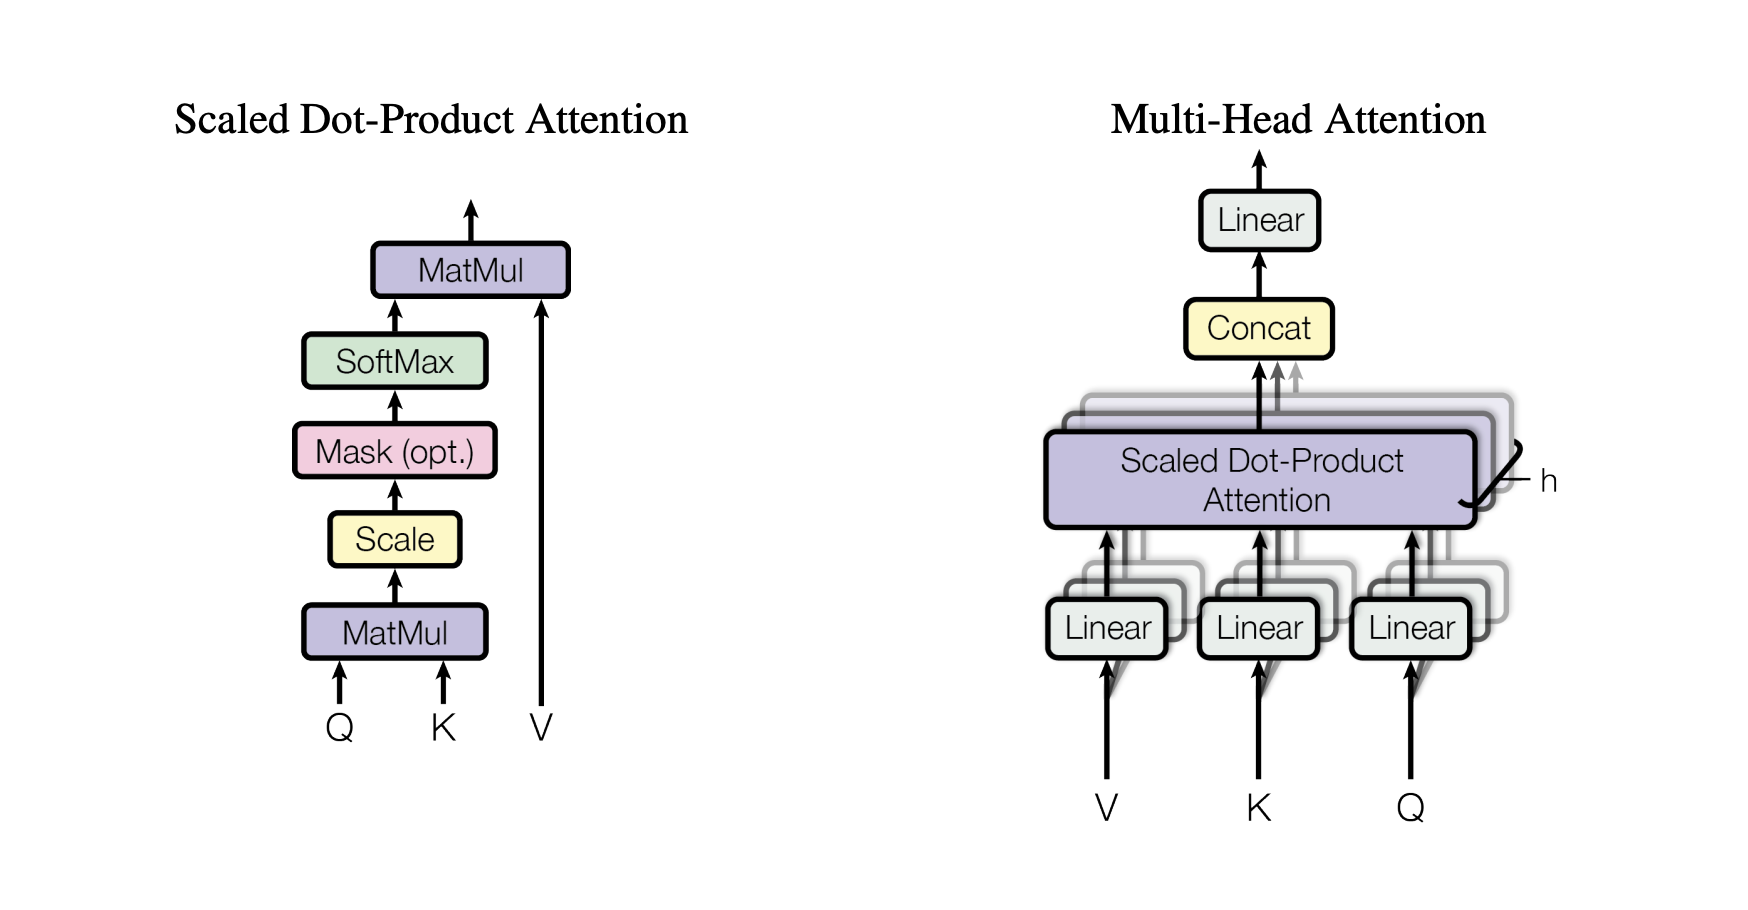
\includegraphics[width=0.9\linewidth]{fig/multi-head.png}
    \caption{Multi-Head Attention consists of several
attention layers running in parallel.}
    \label{fig:enter-label}
\end{figure}

In the original work, the authors chose $h=8$ attention heads. One more important point is that in multi-head attention, usually the $Q, K,$ and $V$ matrices are given to it as input, and there is no need to compute it, unlike in self-attention. However, if they are not provided in the input, they can be taken to be equal to $X$.

\subsection{Transformer Architecture (2017)}

Using the components discussed in the previous section, we can build the Transformer according to the encoder-decoder architecture as seen in figure \ref{fig:transformer}. In the original work, 6 encoder layers and 6 decoder layers were trained.

\begin{figure}[T]
    \centering
    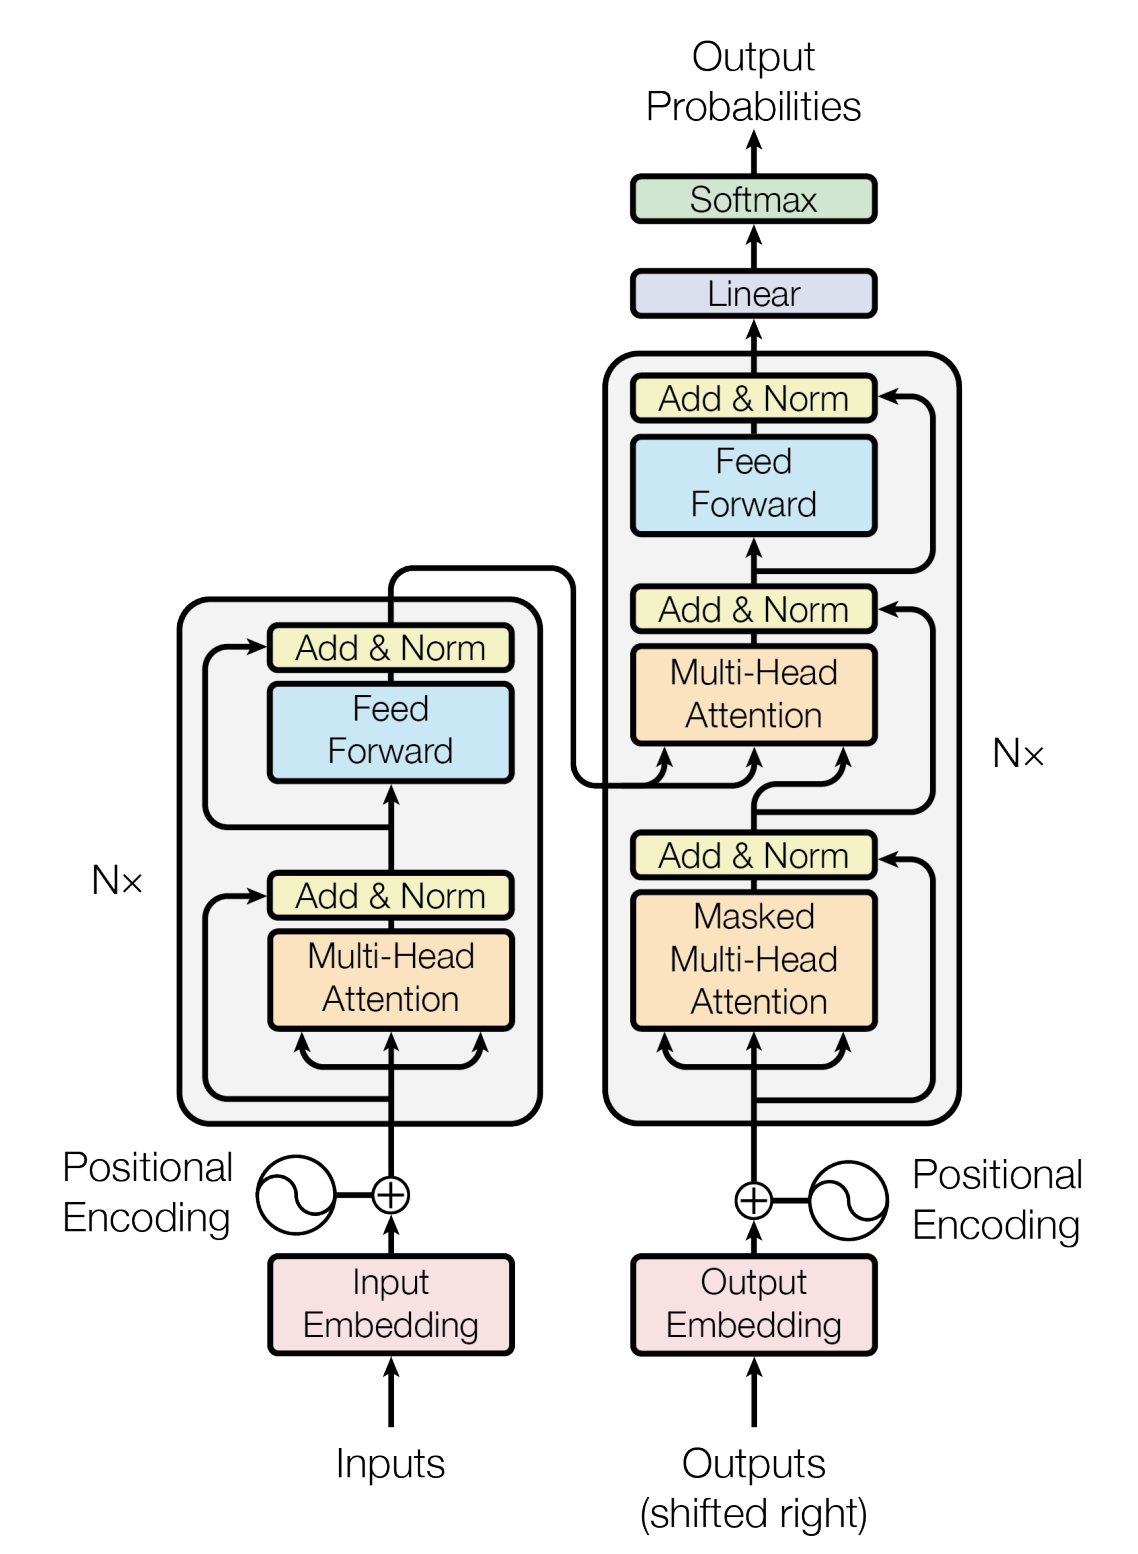
\includegraphics[width=0.65\linewidth]{fig/transfomer.png}
    \caption{Transformer Architecture}
    \label{fig:transformer}
\end{figure}

\subsection{Impact of Transformers}
Transformers were able to achieve state-of-the-art performance compared to the recurrent models. 
Ever since their introduction in 2017, Transformers have revolutionized the field of natural language processing and machine learning as a whole. 

Transformers became the foundation for a wave of groundbreaking models, such as BERT, GPT, and T5, which pushed the boundaries of tasks like translation, summarization, question answering, and text generation. The architecture also extended beyond NLP, impacting areas such as computer vision (e.g., Vision Transformers), time-series analysis, and even protein structure prediction (e.g., AlphaFold \textcolor{red}{[Reference]}). The introduction of pre-training and fine-tuning paradigms further solidified their impact, making domain adaptation efficient and accessible.

\section{Pre-Trained Models and Fine-Tuning}
Given the previous overview on Transformers, two fundamental concepts in NLP are pre-training and fine-tuning language models such as the Transformer. In most of the state-of-the-art language models seen today, these two concepts are used.

\subsection{Pre-Training}
Pre-training is the process of training a model on a large corpus of unlabeled data to learn a general-purpose understanding and representation of the language. This step typically uses self-supervised learning, where the model is trained to predict parts of the input based on the rest, without requiring manually labeled datasets.

Some tasks used for the self-supervised learning in pre-training include:

\begin{enumerate}
    \item \textbf{Masked Language Modeling (MLM):} In MLM, some input tokens are randomly masked, and the model is trained to predict these tokens based on their context. This task was used in the training of BERT\footnote{Bidirectional encoder representations from transformers}  model by Google in 2018 \textcolor{red}{[Reference]}.

    \item \textbf{Causal Language Modeling (CLM):} The model predicts the next token in a sequence given its previous tokens, operating in an autoregressive\footnote{Left-to-right} fashion. GPT\footnote{Generative pre-trained transformer} (2018) by OpenAI uses this approach, training models left-to-right.
\end{enumerate}

Pre-training allows for the learning of syntactic and semantic patterns of the language. These pre-trained models are then used as a foundation, significantly reducing the labeled data requirements for downstream tasks. In the larger pre-trained models improvement of performance can be achieve on diverse tasks.

\subsection{Fine-Tuning}
After pre-training is complete \textbf{Fine-tuning} is performed on a pre-trained model to purpose it for a specific task using labeled data. This step typically modifies the pre-trained weights slightly to optimize performance for the target task.

Transitioning from the pre-training and fine-tuning paradigms, we will explore BERT and GPT which are successful examples of using transformers as pre-trained models and then fine-tuning them to achieve great performance across NLP tasks.

\subsection{GPT (2018)}
GPT (Generative Pre-Trained Transformer) as the names suggest was a pre-trained model based on the decoder of the transformer introduced in 2018.  It introduced unsupervised pre-training followed by supervised fine-tuning. This model uses a unidirectional next word prediction task for training the model on multiple stacks of transformer decoders.

This pre-trained could then be fine-tuned by an output layer or component to specific NLP tasks such as question answering, translation, or text classification.

GPT was trained on the BooksCorpus dataset (a collection of about 11,000 unpublished books) and other publicly available datasets.

Here are some of the specifications of the GPT:

\begin{table}[H]
\centering
\renewcommand{\arraystretch}{1.5}
\setlength{\tabcolsep}{10pt}
\begin{tabular}{@{}lcc@{}}
\toprule
\textbf{Specification}          & \textbf{GPT (2018)}      \\ \midrule
Number of Transformer Layers    & 12                           \\
Number of Parameters            & 117M                         \\
Number of Multi-Head Attentions & 12                           \\ \bottomrule
\end{tabular}
\caption{Specifications of GPT }
\label{tab:gpt_specs}
\end{table}

The GPT achieved state-of-the-art performance in many tasks such as commonsense reasoning and question answering.


\subsection{BERT (2018)}

\begin{figure}[H]
    \centering
    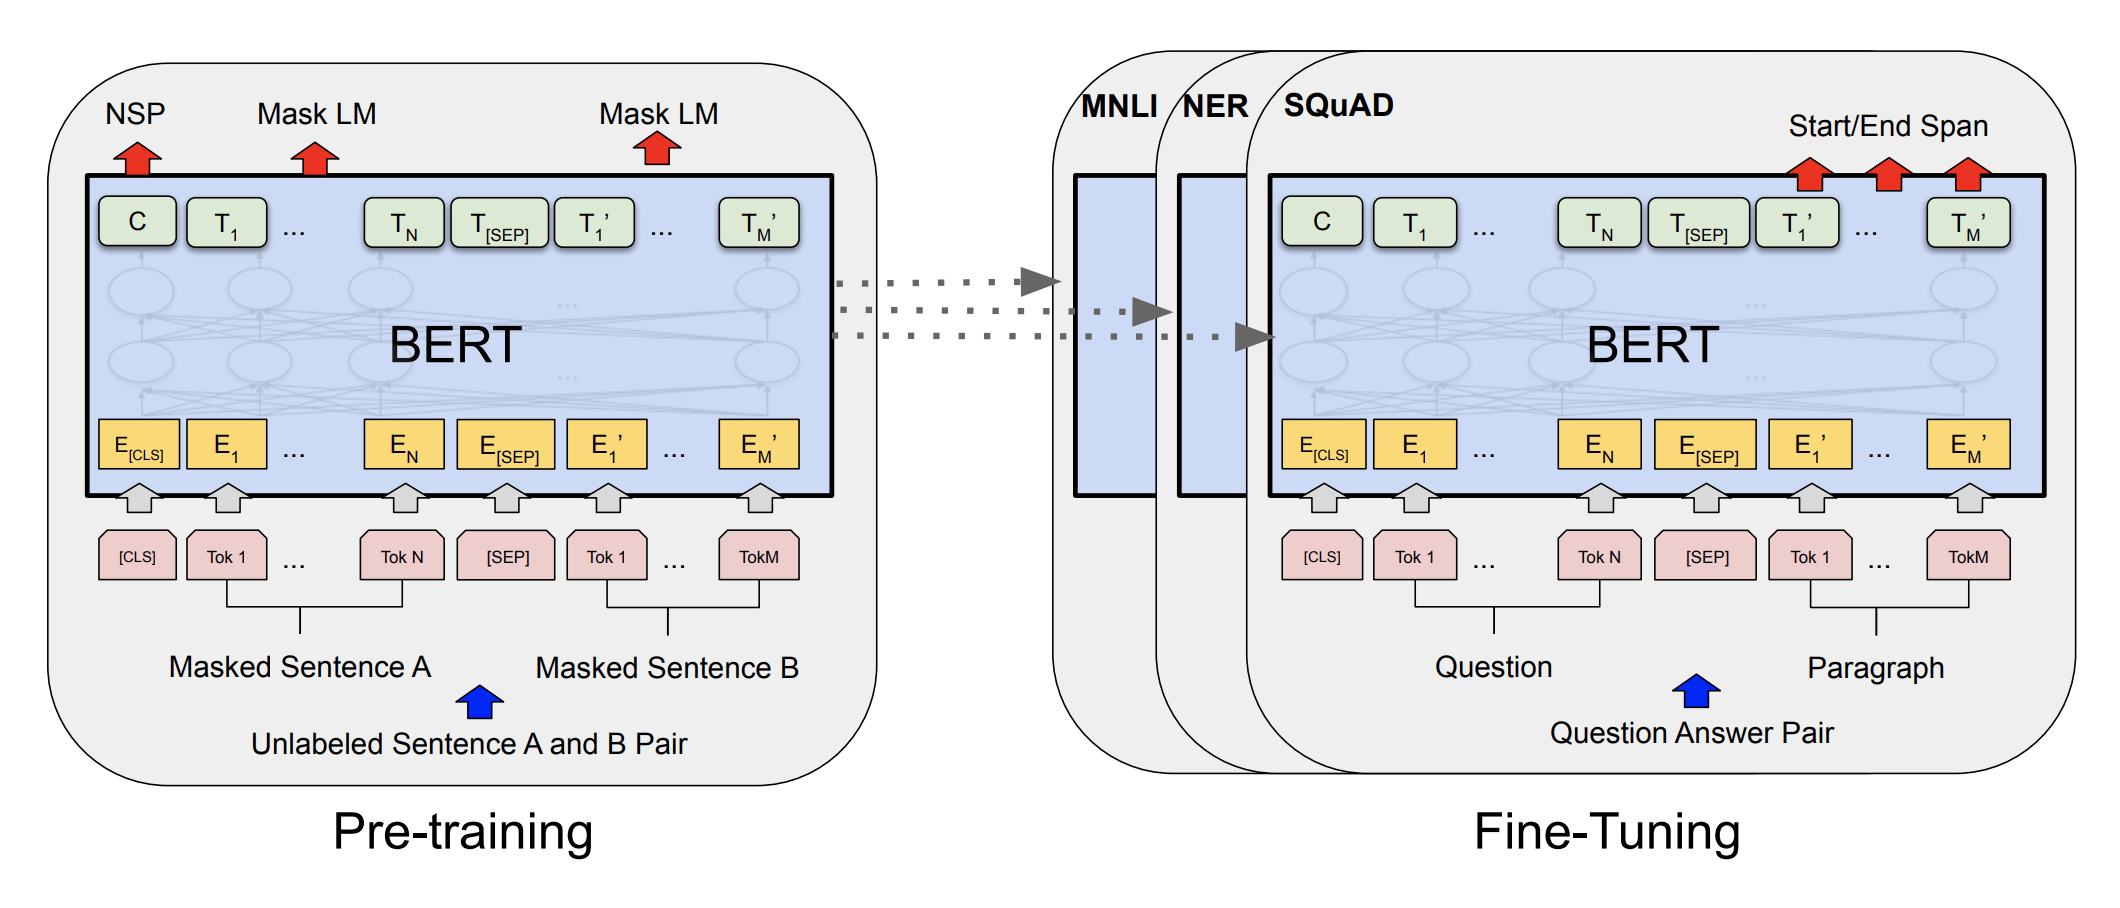
\includegraphics[width=0.9\linewidth]{fig/BERt.png}
    \caption{BERT Training}
    \label{fig:enter-label}
\end{figure}

\textbf{BERT (Bidirectional Encoder Representations from Transformers)} is a pre-trained language model introduced by Google in 2018. Unlike GPT, which is an autoregressive model generating text left-to-right, BERT uses bidirectional language representation by considering both left and right contexts. This bidirectional contextual understanding allows BERT to excel at tasks requiring a comprehensive understanding of the input text, such as classification and question answering.

BERT was pre-trained using only the encoder layer of transformer. One of the innovations of the BERT paper was the masked language model task which allows the model to learn bidirectionally by masking 15\% of the input tokens, either from left or right and asking the model to predict it.

Additionally, next sentence prediction task was also leveraged for model training. This task allows the model to understand the relationship between two sentences. The model is fed pairs of sentences and must predict whether the second sentence is the actual next sentence in the original text. This is particularly useful for tasks like question answering and natural language inference.


There were to versions of BERT released, BERT Base and BERT Large. Here are some specification relating to these two pre-trained models: \\

\begin{table}[H]
\centering
\renewcommand{\arraystretch}{1.5}
\setlength{\tabcolsep}{10pt}
\begin{tabular}{@{}lcc@{}}
\toprule
\textbf{Specification}           & \textbf{BERT-Base} & \textbf{BERT-Large} \\ \midrule
Number of Transformer Layers     & 12                 & 24                  \\
Number of Parameters             & 110M               & 340M                \\
Number of Multi-Head Attentions  & 12                 & 16                  \\ \bottomrule
\end{tabular}
\caption{Specifications of BERT-Base and BERT-Large}
\label{tab:bert_specs}
\end{table}


After pre-training, BERT can be fine-tuned for specific NLP tasks by adding a simple output layer. Fine-tuning adjusts the parameters of BERT slightly to adapt it to the specific task, such as text classification, question answering, named entity recognition, and more.

\section{GPT-2 and GPT-3}

\subsection{GPT 2 (2019)}
In 2019 GPT-2 was introduced. GPT-2 was step up from GPT in terms of its scale. It used a very similar architecture to GPT, however it was much larger which allowed it to have boosted performance across different tasks. It kept the transformer decoder-based self-supervised style of training a pre-trained model and supervised fine-tuning.

It was trained on a dataset of approximately 8 million web pages scraped from the internet (WebText) which was about 40 GB of data.

\subsection{GPT-3 (2020)}
GPT-3 was another state-of-the-art language model developed by OpenAI and released in 2020. It represented a significant advancement over its predecessor, GPT-2, in terms of scale, capabilities, and versatility. It kept the same architecture but yet again increased scale and improved learning methodology.

The model was pre-trained on a massive and diverse dataset of internet text which was about 570 GB large.

The following table shows the specifications of GPT 1 through GPT 3 compared against one another. \\

\begin{table}[H]
\centering
\renewcommand{\arraystretch}{1.5}
\setlength{\tabcolsep}{12pt}
\begin{tabular}{@{}lccc@{}}
\toprule
\textbf{Feature}       & \textbf{GPT-1 (2018)}     & \textbf{GPT-2 (2019)}       & \textbf{GPT-3 (2020)}       \\ \midrule
Layers                 & 12                 & 48                   & 96                   \\
Parameters             & 117M               & 1.5B                 & 175B                 \\
Hidden Size            & 768                & 1600                 & 12,288               \\
Attention Heads        & 12                 & 25                   & 96                   \\
Vocabulary Size        & 40,000             & 50,257               & 50,257               \\
Context Length         & 512                & 1024                 & 2048                 \\ \bottomrule
\end{tabular}
\caption{Specifications of GPT-1, GPT-2, and GPT-3}
\label{tab:gpt_specs}
\end{table}


\subsection{Zero-Shot and Few-Shot Learning}
\textbf{Zero-shot learning} is paradigm where a model generalizes to new tasks or classes without seeing any labeled examples for those tasks during training.

\textbf{Few-shot learning} on the other hand is an approach where an ML model learns to perform a task or classify new classes with only a few labeled examples per class. It leverages prior knowledge from large-scale pretraining or meta-learning to adapt quickly to data-scarce scenarios.

While few-shot learning has been explored conceptually and in limited applications before, the practical realization and broad applicability of few-shot learning in NLP truly started with OpenAI's GPT-3 in 2020. GPT-3 displayed the ability to perform a wide range of tasks by using few-shot prompts, stopping the need for task-specific fine-tuning and changing how language models are used in practice. GPT-3 was capable of this due to its massive size and long training which resulted in a pre-trained model that has learned language representations well enough to be able to perform few-shot learning adequately. In some tasks, few shot learning on GPT-3 performed similarly to models fine-tuned to perform that task. GPT-3 also showed capability of performing zero-shot learning as well.

As an example of few-shot prompts consider the following input to a pre-trained large language model (4-shot prompt):

\hrulefill

\texttt{\textcolor{blue}{Text:} (lawrence bounces) all over the stage, dancing, running, sweating, mopping his face and generally displaying the wacky talent that brought him fame in the first place.
\\
\textcolor{blue}{Sentiment:} positive}

\texttt{\textcolor{blue}{Text:} despite all evidence to the contrary, this clunker has somehow managed to pose as an actual feature movie, the kind that charges full admission and gets hyped on tv and purports to amuse small children and ostensible adults.\\
\textcolor{blue}{Sentiment:} negative
}

\texttt{\textcolor{blue}{Text:} for the first time in years, de niro digs deep emotionally, perhaps because he's been stirred by the powerful work of his co-stars.\\
\textcolor{blue}{Sentiment:} positive}

\texttt{\textcolor{blue}{Text:} i'll bet the video game is a lot more fun than the film. \\
\textcolor{blue}{Sentiment:}
}

\hrulefill

\section{Modern Large Language Models (2020 -- Present)}
\subsection{LLMs}
GPT-3 is an example of a \textbf{large language model}. It is considered ``large" due to its massive amount of parameters (about 175 billion).

To formulate what constitutes an LLM\footnote{Large language model}, we can state some properties LLMs generally have:
\begin{enumerate}
    \item \textbf{They have tens of billions of parameters}, e.g. 1.76 trillion parameters on OpenAI's GPT-4.
    \item \textbf{They are trained on a massive and diverse corpus of text}, e.g. Meta's LLaMA was trained on about 1.4 TBs of text.
    \item  \textbf{They are capable of generalization such as zero-shot and few-shot learning}.
    \item \textbf{They often support a large context window.}
    \item  \textbf{They require significant computational resources for training and inference}, e.g. Google's Gemini Ultra cost about 190 million dollars to train.
\end{enumerate}

Now, we will briefly mention some of the modern LLMs that have taken the world by storm. It will become apparent that most LLMs today are trained in the industry rather than in academia.

\subsection{OpenAI's GPT-3.5 (2022)}
GPT‑3.5 marked a turning point in making large language models broadly accessible. Originally used as the backbone for ChatGPT when it launched in late 2022, GPT‑3.5’s conversational fluency and general-purpose language understanding impressed millions of users who had never before interacted with AI at such scale. Its underlying architecture was an evolution of GPT‑3, the refinement in dialogue management and context awareness made it a favorite for applications ranging from customer support to creative writing. This model’s success helped fuel a wave of public enthusiasm and research investment in conversational AI technologies.

\subsection{OpenAI's GPT-4 (2023)}
Launched in March 2023, GPT‑4 took the capabilities of its predecessor to a new level by incorporating multimodal inputs and improved reasoning skills. It expanded context window and the ability to process both text and images. Its performance improvements on professional exams and coding tasks caused both scientific admiration and commercial hype. GPT‑4’s integration into products like ChatGPT Plus and Bing Chat underscored its market impact and solidified OpenAI’s leadership in generative AI research.

\subsection{Google's Gemini (2023)}
Google’s Gemini released in 2023 as a rival in the race for multimodal intelligence. Designed to handle text, images, and even video, Gemini drew significant attention for its extended context lengths—up to millions of tokens—and robust integration of diverse data types. Gemini’s launch signaled Google’s determination to lead in next‑generation AI systems and sparked widespread debate about the future interplay between AI multimodality and practical application. Although a very powerful model, the market was mostly dominated by OpenAI's models due to their better overall performance and quality.

\subsection{OpenAI's GPT-4o (2024)}
Introduced in May 2024, GPT‑4o (with “o” standing for “omni”) pushed the envelope further by unifying text, image, and audio processing in a single model. Its design emphasized cost‑efficiency and speed while delivering state‑of‑the‑art performance on multilingual and multimodal benchmarks. The model quickly gained hype as it let more natural, humanlike interactions. By significantly reducing the cost per token compared to earlier models, GPT‑4o demonstrated that high‑performance multimodal AI could be both powerful and economically viable.

\subsection{OpenAI's o1 (2024)}
Released in late 2024, OpenAI’s o1 model was a breakthrough in advancing AI reasoning. Unlike its prediction‑only predecessors, o1 was designed to “think” through complex queries using reinforcement learning techniques that allowed it to explore multiple solution paths before giving an answer. This model excelled at challenging tasks in mathematics, coding, and scientific problem solving.

\subsection{Deepseek R1 (2025)}
Deepseek R1, released in January 2025 by a Chinese AI startup, has been regarded as a disruptive force in the AI landscape. This model achieved performance levels comparable to OpenAI’s advanced o1 series while costing a fraction of the price. This achievement has been regarded as an “AI Sputnik moment.” More importantly Deep Seek R1 is an open-source model unlike its OpenAI counterparts. Its release has caused intense discussion about international competitiveness in AI research. By demonstrating that reasoning and natural language understanding can be achieved with less costly training, Deepseek R1 has pushed scientific boundaries and reshaped market expectations for future AI development.





\end{document}
